Digitale kretser består av binære systemer.
De består av komponenter som kan ha tilstand 1 eller 0.
Logikken i disse kretsene kommer fra boolsk algebra,
og komponentene de bygges av kalles for \emph{logiske porter}.
\\
Det finnes en del forskjellige logiske porter, men alle disse kan lages
ved å kombinere 3 grunnlegende typer:
NOT, AND og OR.



\subsubsection{NOT, AND og OR}
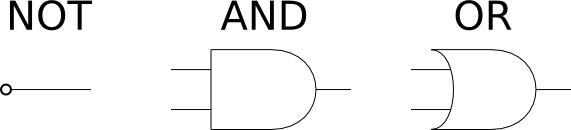
\includegraphics[width=0.67\textwidth]{./img/notandor}
\\\\
NOT: Inverterer signalet.
     Hvis det er en input, er det ingen output.
     Hvis det ikke er input, er det en output.
\\
AND: Begge signalene inn må være på for å få output.
\\
OR:  Enten den ene eller den andre (eller begge) gir output.



\subsubsection{Andre typer}
Ved f.eks. å kombinere NOT og AND får man en NAND.
Det samme gjelder for NOR.
\\
Det finnes også en XOR som er helt lik OR bortsett fra at
begge signalene kan ikke være på samtidig.
X står for exclusive.
\\\\
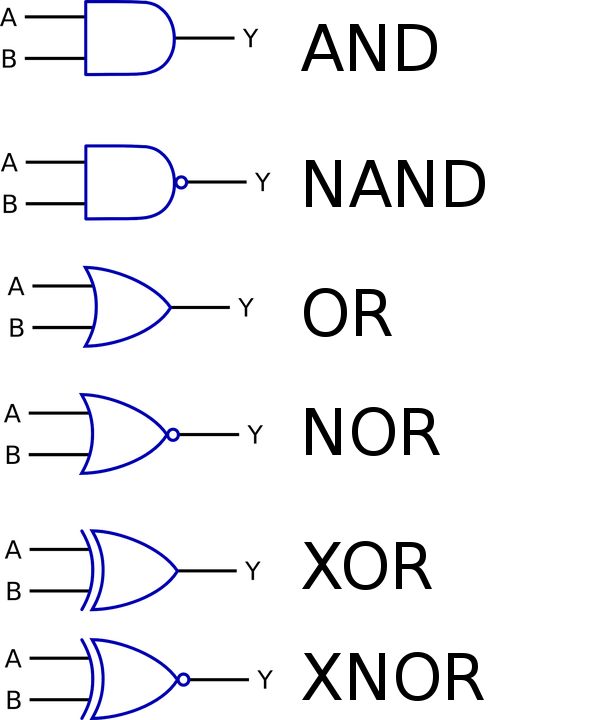
\includegraphics[width=0.5\textwidth]{./img/gatesymbols}



\subsubsection{Sannhetstabell (truth table)}
Output fra en logisk port avhenger av input og varierer fra port til port.
En sannhetstabell gir oversikt over hvilke porter som gjør hva.
\\\\
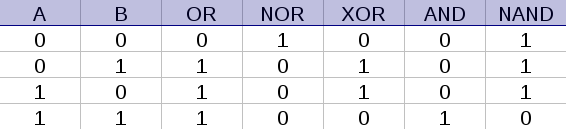
\includegraphics[width=\textwidth]{./img/truthtable}
